\scanpage{15}
\mspage{5}

impliquent
\[
\text{b')}\quad\varphi_!(F\times G)\longrightarrow\varphi_!(F)\times\varphi_!(G)\quad\text{épi}
\qquad\forall F,G\text{ dans }\operatorname{Ob}\widehat A
\]
\[
\text{c')}\quad\varphi_!(G\times_F H)\longrightarrow
\varphi_!(G)\times_{\varphi_!(F)}\varphi_!(H)\quad\text{épi}
\]
$\forall$ diagramme
\diagram{\begin{tikzcd}[ampersand replacement=\&,column sep=small,row sep=small]
G\arrow[dr]\&\&H\arrow[dl]\\
\&F\&
\end{tikzcd}}
dans $\widehat A$.

et de là, plus généralement, la forme équivalente \unsure{unique} de Hyp 1, 2, 2' :

\figure{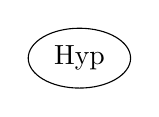
\begin{tikzpicture}\draw (0,0) ellipse (.65 and .38);\node at (0,0) {Hyp};\end{tikzpicture}}
Pour tout diagramme fini $(F_i)_{i\in I}$ dans $\widehat A$, la flèche canonique
\[
\varphi_!\left(\varprojlim_I F_i\right)\longrightarrow\varprojlim_I\varphi_!(F_i)
\]
est épi.

(Il suffit d'ailleurs de le postuler quand les $F_i$ sont dans $A$, et dans les trois cas particuliers $I=\bullet$, $\bullet\ \bullet$,
\diagram{\begin{tikzcd}[ampersand replacement=\&,column sep=tiny,row sep=tiny]
\bullet\arrow[dr]\&\&\bullet\arrow[dl]\\
\&\bullet\&
\end{tikzcd}}, correspondants aux axiomes Hyp 1, Hyp 2, Hyp $\unsure{2|1}'$.)

Mais cette hypothèse peut-elle être vérifiée, sans que $\varphi_!$ soit $=$ ex.\textsuperscript{t} à gauche ?

\margin{14}
